\documentclass[10pt,french,french]{article}
\usepackage{lmodern}
\usepackage{amssymb,amsmath}
\usepackage{ifxetex,ifluatex}
\usepackage{fixltx2e} % provides \textsubscript
\ifnum 0\ifxetex 1\fi\ifluatex 1\fi=0 % if pdftex
  \usepackage[T1]{fontenc}
  \usepackage[utf8]{inputenc}
\else % if luatex or xelatex
  \ifxetex
    \usepackage{mathspec}
    \usepackage{xltxtra,xunicode}
  \else
    \usepackage{fontspec}
  \fi
  \defaultfontfeatures{Mapping=tex-text,Scale=MatchLowercase}
  \newcommand{\euro}{€}
\fi
% use upquote if available, for straight quotes in verbatim environments
\IfFileExists{upquote.sty}{\usepackage{upquote}}{}
% use microtype if available
\IfFileExists{microtype.sty}{%
\usepackage{microtype}
\UseMicrotypeSet[protrusion]{basicmath} % disable protrusion for tt fonts
}{}
\usepackage[margin=0.80in]{geometry}
\ifxetex
  \usepackage{polyglossia}
  \setmainlanguage{}
\else
  \usepackage[shorthands=off,french]{babel}
\fi
\usepackage{longtable,booktabs}
\ifxetex
  \usepackage[setpagesize=false, % page size defined by xetex
              unicode=false, % unicode breaks when used with xetex
              xetex]{hyperref}
\else
  \usepackage[unicode=true]{hyperref}
\fi
\hypersetup{breaklinks=true,
            bookmarks=true,
            pdfauthor={},
            pdftitle={},
            colorlinks=true,
            citecolor=blue,
            urlcolor=blue,
            linkcolor=magenta,
            pdfborder={0 0 0}}
\urlstyle{same}  % don't use monospace font for urls
\setlength{\parindent}{0pt}
\setlength{\parskip}{6pt plus 2pt minus 1pt}
\setlength{\emergencystretch}{3em}  % prevent overfull lines
\setcounter{secnumdepth}{5}

\providecommand{\tightlist}{%
  %\setlength{\itemsep}{0pt}
  \setlength{\parskip}{0pt}
  }

%%% Use protect on footnotes to avoid problems with footnotes in titles
\let\rmarkdownfootnote\footnote%
\def\footnote{\protect\rmarkdownfootnote}


  \title{~\textsc{note de synthèse}\\
\hspace*{0.333em}\emph{Word-Embedding} et sentiments des ménages avec
Twitter}
    \author{Kim Antunez, Romain Lesauvage, Alain Quartier-la-Tente\\
sous l'encadrement de Benjamin Muller (Inria)}
    \date{}
  
\usepackage[T1]{fontenc}
\usepackage{caption}
\usepackage{graphicx}
\usepackage{natbib}
\usepackage[dvipsnames]{xcolor}
\usepackage{fontawesome5}
\DeclareMathOperator{\arctanh}{arctanh}
\usepackage{subcaption}
\usepackage{amsfonts}
\usepackage{dsfont}
\usepackage{xspace}
\usepackage{enumitem}
\usepackage{pifont}
\usepackage{wrapfig}
\usepackage{textpos}
\usepackage{array}
\usepackage{multicol}


\usepackage[tikz]{bclogo}
\newcounter{comptEncadre}
\renewcommand\thecomptEncadre{%\thesection.
\arabic{comptEncadre}}
\definecolor{processblue}{cmyk}{0.96,0,0,0}
\newenvironment{encadre}[2][false]{\refstepcounter{comptEncadre}
      %\addcontentsline{exp}{encadres}{\protect\numberline{\thecomptEncadre}#1}%
\begin{bclogo}[couleur=processblue!5,arrondi=0.1,
logo=\bcloupe,barre=none,couleurBord=blue!60!green,nobreak = #1]{ {\sc \textbf{Encadré \thecomptEncadre}} -  #2}
\smallskip
}{\end{bclogo}}

\begin{document}

\maketitle


\begin{textblock*}{\textwidth}(0cm,-7.5cm)
\begin{center}

\includegraphics[height=2.5cm]{img/LOGO-ENSAE.png}
\end{center}
\end{textblock*}

Grâce à l'évolution des méthodes d'apprentissage profond (\emph{Deep
Learning}), l'appréhension du langage naturel est aujourd'hui devenue
une discipline à part entière (\emph{Natural Language Processing}). Ce
succès s'explique en partie grâce à l'émergence de techniques non
supervisées d'apprentissage de représentation de structures
linguistiques. Les méthodes de \emph{word-embedding} («~plongement
lexical~» en français) permettent de représenter chaque mot d'un
dictionnaire par un vecteur de nombres réels afin que les mots qui
apparaissent dans des contextes similaires possèdent des vecteurs
correspondants qui sont relativement proches (au sens d'une distance
définie). Les variantes du modèle \emph{word2vec}, développé par une
équipe de recherche chez Google, sont parmi les plus célèbres.

En partie \ref{sec:word2vec}, nous décrivons le modèle \emph{word2vec}
que nous avons implémenté grâce à la librairie \texttt{Pytorch} de
Python. Au-delà de la compréhension du modèle, nous nous sommes
également initiés aux tests d'hyperparamètres et à son évaluation sur un
corpus fictif (partie \ref{sec:evaluation}) grâce à plusieurs méthodes
(calculs de similarités cosinus, opérations vectorielles sur les mots,
méthodes de réduction de dimension ACP et t-SNE et jugement humain). Il
a été fascinant d'observer à quel point le modèle présente d'excellents
résultats en termes de capture sémantique des mots dans un texte.

Dans la partie \ref{sec:sentimentalAnalysis}, nous avons cherché à
construire un indice mensuel de sentiment des tweets et à le comparer
aux indicateurs produits dans la statistique publique. L'entraînement et
le test d'un modèle logit dont les prédicteurs correspondent aux
dimensions des \emph{word-embeddings} nous a permis de remarquer qu'en
plus de représenter la proximité entre mots, le modèle \emph{word2vec}
permet de capter dans une certaine mesure le sentiment de phrases.

\begin{figure}[htb]
\tikzstyle{myboxnorm} = [very thick,
    rectangle, rounded corners, inner sep=2pt, inner ysep=3pt, right,
    align=center]
\tikzstyle{myboxw2v} = [draw=red!50, fill=orange!10, myboxnorm]
\tikzstyle{myboxmod} = [draw=blue!60!green, fill=blue!5, myboxnorm]
\tikzstyle{myboxcomp} = [draw=green!50!black, fill=green!5, myboxnorm]

\tikzstyle{titlenorm} = [fill=white, very thick,
    rectangle, inner sep=2pt, inner ysep=2pt,font=\bfseries,
    text width=4.2cm, above=-0.3cm, align=center,
    minimum height=1.15cm]
\tikzstyle{titlew2v} = [draw=red!50, text = red!50,titlenorm]
\tikzstyle{titlemod} = [draw=blue!60!green,text=blue!60!green,titlenorm]
\tikzstyle{titlecomp} = [draw=green!50!black,text=green!50!black, titlenorm]    

\tikzstyle{fleche} = [->,rounded corners,line width=1pt]

\begin{tikzpicture}
\usetikzlibrary{fit}
\usetikzlibrary{arrows.meta}
%Il faut d'abord faire les boites
% w2vec
\node[fit={(2.5,1.5) (-3.,-3.5)}, myboxw2v,semitransparent] (w2vrect) {};
\node[fit={(2.7,1.5) (8.2,-5.5)}, myboxmod,semitransparent] (rectmod) {};
\node[fit={(13.9,1.5) (8.4,-5.5) }, myboxcomp,semitransparent] (rectcomp) {};

\node at (0,0) [myboxw2v] (tweets) {Tweets};
\node at (2.4,0) [myboxw2v] (we) {\textit{word-embedding}};
% sentiment
\node at (0,-4.5) [myboxnorm,text width=2.5cm, draw = black] (bddsent) {Échantillon de tweets annotés
};

% analyse de sentimentsentiment
\node at (7,0) [myboxmod] (logit) {Modèle logit};
\node at (7,-4.5) [myboxmod,text width=2.22cm] (baseline) {Modèle lexical};

% analyse de sentimentsentiment
\node at (12,0) [myboxcomp,text width=3.8cm] (indsent) {Indices mensuels de \\sentiment des tweets};

\node at (12,-4.5) [myboxcomp,text width=3.8cm] (camme) {Indicateur synthétique \\de confiance des

ménages (Insee)};

%Fleches
\draw[fleche] (tweets.east) --(we.west) node[below = 0.2cm,pos=1]{
\begin{minipage}{5cm} \footnotesize
  \begin{itemize}[label=\scalebox{.6}{\ding{110}}] 
  \item tokénisation
  \item choix hyperparamètres
  \item évaluation : 
  \begin{itemize}[label=\scalebox{.6}{\ding{117}}]
    \item similarité cosinus
    \item réduction de dimension (ACP/TSNE)
    \item jugement humain
  \end{itemize}
  \end{itemize} 
\end{minipage} 
};
\draw[fleche] (bddsent.east)--(baseline.west) 
  node[pos=0.36,text width=3cm]{
    \footnotesize bases  
    
    test/entraînement}
  node[pos=0.96, below = 0.05cm,text width=2.5cm]{
    \footnotesize sentiment 
    
    moyen d'un mot};
\draw[fleche] (bddsent.east)--++(2,0)--++(0,0.8)-|(logit.south);
\draw[fleche] (we.east)--(logit.west)node[pos=0.89,text width=2.5cm]{\footnotesize \emph{sentence}
  
  \emph{embedding}};
\draw[fleche] (logit.east)--
  (indsent.west)node[pos=0.62,text width=2.5cm]{\footnotesize moyennes
  
  mensuelles};
\draw[fleche] (baseline.east)-|(9.6,0)--(indsent.west);
\draw[fleche,<->] (indsent.south)--(camme.north) 
  node[pos=.5,text width=2.5cm, right=0.2cm]{\footnotesize distance entre
  
  indicateurs}
  node[pos=.5,text width=1.7cm, left]{\footnotesize prévision /
  
  causalité};

\node[titlew2v] at (w2vrect.north) { word2vec \\
(skip-gram)};
\node[titlemod] at (rectmod.north) { Analyse de \\
sentiment d'un tweet};
\node[titlecomp] at (rectcomp.north) { Comparaison \\
d'indices mensuels};
\end{tikzpicture}
\end{figure}

Bien que l'indice obtenu s'avère utile pour prédire l'indicateur
synthétique de confiance des ménages (Camme, Insee), les différences
observées entre les deux séries demeurent importantes en raison de leurs
philosophies différentes et des limites de la base d'entraînement de
tweets annotés (\emph{domain-shift}, processus d'annotation, mots
inconnus) qui invitent à des pistes d'amélioration (prétraitement plus
approfondi des tweets, modèles d'analyse de sentiment plus
élaborés\dots).

\newpage

\section{\texorpdfstring{Implémentation du modèle
\emph{word2vec}}{Implémentation du modèle word2vec}}\label{sec:word2vec}

Les modèles \emph{word2vec}, développés par une équipe de recherche chez
Google, sont parmi les plus célèbres modèles de \emph{Natural Language
Processing} qui utilisent le \emph{word-embedding} --- plongement
lexical en français. Il s'agit de représenter chaque mot par un vecteur
dont la dimension est fixée par la valeur d'un hyperparamètre.

\begin{wrapfigure}[15]{r}[0pt]{0cm}
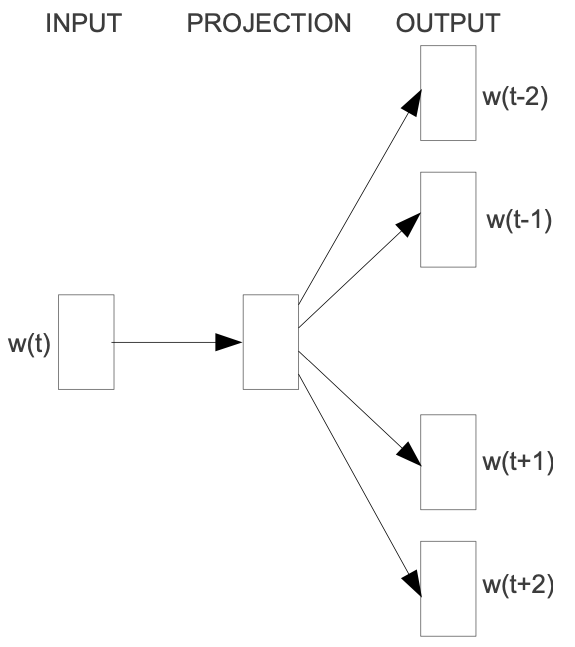
\includegraphics[width=5cm]{img/skip_gram.png}
\captionsetup{margin=0cm,format=hang,justification=justified}
\caption{Architecture\newline du modèle Skip-gram.}\label{fig:skipgram}
\end{wrapfigure}

L'approche \emph{Skip-gram} a pour objectif d'estimer, pour chaque mot
du vocabulaire qualifié de \textbf{«~contexte~»}, la probabilité d'être
proche d'un mot qualifié de \textbf{«~focus~»} (figure
\ref{fig:skipgram}). Ainsi, les mots qui apparaissent dans des contextes
similaires («~bonjour~» et «~salut~» par exemple) seront représentés par
des vecteurs relativement proches dans l'espace vectoriel de définition
de ces vecteurs.

Pour transformer chaque mot en un vecteur, nous entraînons un réseau de
neurones sur une tâche annexe : on construit un classifieur dont la
tâche de prédiction est binaire pour chacun des mots du vocabulaire et
répond à la question «~Est-ce que ce mot contexte est susceptible d'être
voisin du mot focus ?~». Ce n'est pas la prédiction en elle-même qui
nous intéresse, mais plutôt le poids du classifieur en sortie du modèle
qui correspondra aux \emph{word-embeddings} de dimension \(dim\).

\emph{Skip-gram} est un réseau de neurones à deux couches avec deux
matrices initialisées en générant des lois normales \(\mathcal N(0,1)\)
:

\begin{itemize}
\item
  En entrée une matrice \(W_e\) de taille \(n\times dim\) ;
\item
  En sortie une matrice \(W_s\) de taille \(n\times dim\).
\end{itemize}

Nous entraînons le réseau de neurones en le nourrissant de paires
\texttt{{[}focus,\ contexte{]}} contenues dans les \(n\) mots du
vocabulaire des tweets. Pour cela, on tire au hasard\footnote{Pour
  éviter que les mots trop fréquents, souvent peu informatifs, soient
  sur-entraînés, on effectue tout d'abord un sous-échantillonnage
  (\emph{subsampling}).} un mot focus pour lequel on tire un mot
\emph{contexte} au hasard dans une fenêtre \(w\). Ce mécanisme va être
répété sur toutes les phrases du corpus et l'ensemble du corpus va être
parcouru plusieurs fois. Le nombre de fois que l'ensemble du corpus est
parcouru est appelé \emph{epochs}.

À chaque étape, les matrices sont mises à jour par descente de gradient
:

\[\theta^{(t+1)} = \theta^{(t)} - \eta \nabla_\theta Loss(\theta^{(t)})\]

avec \(\eta\) le taux d'apprentissage et \(Loss(\theta)\) la fonction de
perte.

Le modèle \emph{word2vec} a initialement été construit en utilisant une
fonction de perte dérivée de la fonction \emph{softmax}. L'inconvénient
de cette méthode est qu'elle est très gourmande en temps de calcul
(\(\mathcal O(n)\) par phrase). L'algorithme a donc ensuite été amélioré
en utilisant le \emph{negative sampling}. Dans cette approche, on
utilise une fonction de perte sigmoïde. De plus, plutôt que de mettre à
jour l'ensemble des représentations vectorielles des mots pour chaque
couple \texttt{{[}focus,\ contexte{]}}, on tire \(K\) mots au hasard du
vocabulaire \((w_{neg,\,i})_{i=1..K}\) en considérant que ces mots ne
seront pas des mots voisins de \texttt{focus}. La complexité est ici
bien plus faible que pour la fonction \emph{softmax} (\(\mathcal O(K)\)
par phrase), ce qui correspond à un gain considérable en termes de temps
de calcul.

À la fin de l'algorithme, ce sont ces matrices qui donneront la
représentation vectorielle des mots du vocabulaire. Ainsi, la ligne
\(i\) de la matrice \(W=\frac{W_e+W_s}{2}\) donnera la représentation du
\(i\)\textsuperscript{ème} mot du vocabulaire en dimension \(dim\).

\newpage

\section{Évaluation du modèle implémenté}\label{sec:evaluation}

Malgré l'utilisation généralisée des \emph{word embeddings}, très peu de
travaux théoriques expliquent ce qui est réellement capturé par ces
représentations de mots. C'est pourquoi nous avons évalué la qualité des
vecteurs-mots obtenus en sortie de notre modèle \emph{word2vec} à l'aide
de méthodes empiriques : la similarité cosinus entre deux mots, la
réduction de dimension de l'espace des vecteurs-mots (ACP, t-SNE) et
l'évaluation par jugement humain.

Grâce à l'évaluation de plusieurs modèles, nous avons pu déterminer les
hyperparamètres les plus pertinents \footnote{
$ep = 100$ pour le nombre d'\og \emph{epochs} \fg / $lr = 0,02$ pour le \og \emph{learning rate} \fg, ou taux d'apprentissage/ $w = 4$ pour la taille de la fenêtre (\emph{window}) de sélection des mots contextes / $dim = 100$ pour la dimension des vecteurs-mots (ou \emph{word-embeddings}).
} au regard des données dont nous disposons (encadré
\ref{enc:encadre1}). Selon nos critères d'évaluation, les résultats
obtenus en sortie du modèle \emph{word2vec} nous confirment la qualité
de l'entraînement du corpus de 1,3 million de tweets\footnote{Avant de
  nous attaquer au jeu de données complet, nous avons également évalué
  notre modèle sur un corpus fictif afin de nous assurer de sa
  robustesse et de sa validité.} :

\begin{itemize}
\item Le coefficient de corrélation de Spearman avec le jugement humain est significatif (p-valeur proche de 0 \%) et assez élevé (0,495).
\item La recherche des plus proches voisins par similarité cosinus donne des résultats proches de l'intuition pour quelques mots de référence évalués (bonjour, femme, samedi\dots).
\item La projection de certains vecteurs-mots sur les deux premiers axes d'une ACP (figure \ref{fig:acp_gensim}) est de qualité.
\item Les sommes vectorielles sur les vecteurs-mots présentent des résultats plus mitigés. L'exemple de  $\overrightarrow{Roi} - \overrightarrow{Homme} + \overrightarrow{Femme} = \overrightarrow{Reine}$ (figure \ref{fig:acp_reine}) semble plutôt fonctionner. 
\end{itemize}

\begin{figure}[h]
\begin{minipage}{.5\textwidth}
\centering
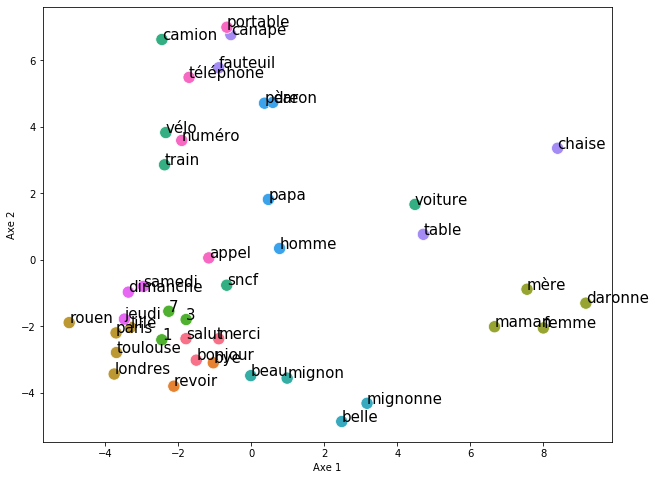
\includegraphics[width=0.77\textwidth]{img/acp_gensim.png}
\captionsetup{margin=0cm,format=hang,justification=justified}
\caption{ACP sur un corpus réduit de mots.}\label{fig:acp_gensim}
\end{minipage}%
\begin{minipage}{.5\textwidth}
   \centering
  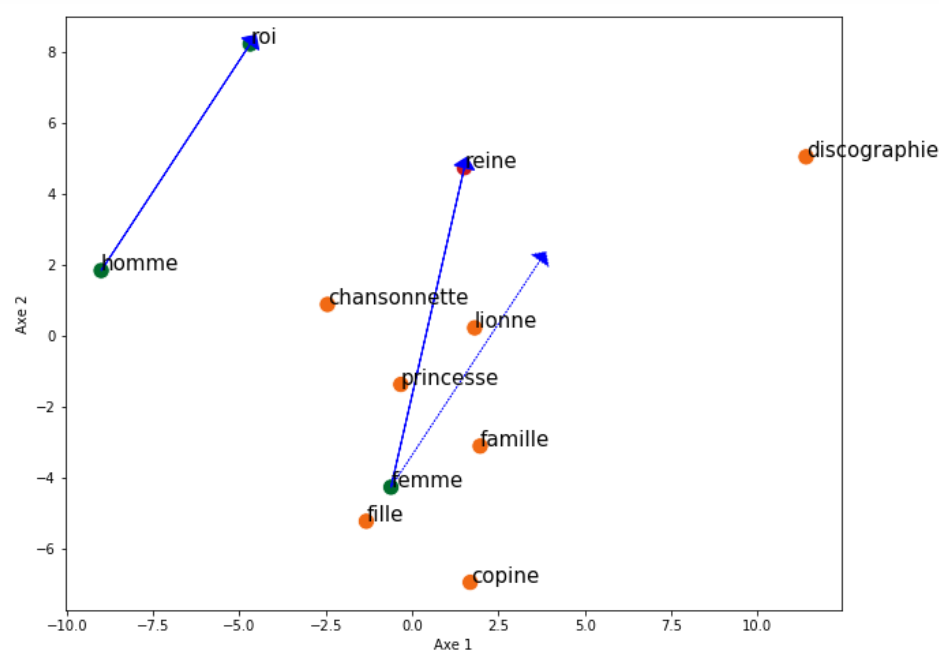
\includegraphics[width=0.8\linewidth]{img/acp_reine.png}
  \captionof{figure}{\ $\protect\overrightarrow{Roi} - \protect\overrightarrow{Homme} + \protect\overrightarrow{Femme} = $ ?}
  \label{fig:acp_reine}
\end{minipage}%
\end{figure}

\begin{encadre}[true]{Données utilisées}\label{enc:encadre1}

\small

\textbf{Tweets postés en France entre 2011 et 2018}

Ces données correspondent à un ensemble de tweets postés en France entre 2011 et 2018, supposés être représentatifs de l'ensemble de tweets nationaux publiés durant cette période. \\
Pour entraîner notre modèle \emph{word2vec}, nous avons mobilisé un premier échantillon de 1,3 million de tweets. Un second échantillon, composé de 4 200 tweets mensuels sur la période 2011-2018, a été utilisé pour construire notre indice mensuel de sentiment. 

\textbf{Tweets annotés sur les transports urbains}

Cette base est composée d'un ensemble d'environ 23 000 tweets qui concernent les transports urbains (trains SNCF, métros et bus de la RATP) annotés en termes de sentiment ($1$ s'ils sont positifs, $0$ s'ils sont négatifs).\\
Elle a été utilisée pour entraîner notre modèle d'analyse de sentiment.

\textbf{Indicateur synthétique de confiance des ménages}

L’indicateur synthétique de confiance des ménages provient de l'Enquête mensuelle de conjoncture auprès des ménages (Camme) de l’Insee.\\
C'est l'indicateur que nous cherchons à prévoir à partir de notre indice mensuel de sentiment.

\end{encadre}

\newpage

\section{Construction d'un indice mensuel de sentiment moyen des
tweets}\label{sec:sentimentalAnalysis}

Nous utilisons ici les vecteurs-mots en sortie du modèle
\emph{word2vec}, couplés avec une base de tweets qui concernent les
transports urbains qualifiés de positifs ou négatifs, afin de créer un
indice mensuel de sentiment moyen des tweets.

Nous cherchons tout d'abord à construire un modèle permettant de prédire
le sentiment (\(0\) si négatif ou \(1\) si positif) associé à un tweet à
partir des mots qui le composent. Nous comparons les deux modélisations
suivantes en évaluant leur efficacité. Pour cela, la base de tweets
annotés sur les transports a été séparée en une base d'entraînement
(environ 16 000 tweets) et une base de test (environ 7 000 tweets).

\begin{multicols}{2}

\textbf{Modèle lexical : sentiment moyen des mots }

Ce premier modèle de prédiction du sentiment utilise l'information des tweets labelisés pour déterminer un sentiment moyen par mot.
Le sentiment prédit d'un tweet $t$ composé de $n$ mots sera :
$$S_{1,\gamma}(t) = \mathds{1}\left\{ \frac{1}{n} \sum \limits_{i=1}^n \alpha_i \geq \gamma\right\} \qquad \in \{ 0,1\}$$
  avec $\gamma \in [-1,1]$ un seuil fixé, $\alpha_i = \frac{nb_+(i) - nb_-(i)}{nb_+(i) + nb_-(i)} \in [-1,1]$  le sentiment moyen du mot $i$ calculé à partir du nombre de tweets positifs ($nb_+(i)$) et négatifs ($nb_-(i)$) dans lesquels il apparaît.

\vspace{2.5cm}

\textbf{Modèle logit : \emph{word-embeddings}}

Ce deuxième modèle est une régression binaire avec comme prédicteurs chacune des 100 dimensions des vecteurs-mots. Les vecteurs-mots sont moyennés pour obtenir la représentation vectorielle du tweet : la  « \emph{sentence-embedding} ».
Le sentiment prédit d'un tweet $t$ sera :
 $$S_{2,\gamma}(t) =\mathds{1}\left\{   \mathbb{P}(Y_i = 1 | X_{i}) \ge \gamma\right\} \qquad \in \{ 0,1 \}$$
Avec : 
\footnotesize{
$$Y_i = \mathds{1}\left\{ \sum_{i = 1}^n \beta_i X_{i,j} + \varepsilon_i \geq 0 \right\} \quad  \mathbb{P}(Y_i = 1 | X_{i}) = F_{\varepsilon}\left(\sum_{i = 1}^n \beta_i X_{i,j}\right)$$
}

\normalsize
\begin{itemize}
\item $Y_i$ le sentiment du tweet $i$ ;
\item $X_{i,1}, \dots, X_{i,n}$ les coordonnées de la \emph{sentence-embedding} du tweet $i$ ;
\item $\varepsilon_i$ le résidu de notre modèle de fonction de répartition $F_{\varepsilon}(x) = \frac{1}{1 + e^{-x}}$ (logit).
\end{itemize}

 \end{multicols}

\begin{multicols}{2}
\faArrowCircleRight{} \emph{Accuracy}\footnote{Taux de tweets dont le sentiment est bien prédit.} =  89,1 \% ($\gamma^* = -0,14$).

\faArrowCircleRight{} \emph{Accuracy} =  69,8 \% ($\gamma^* \simeq 0,5$).

 \end{multicols}

À partir de ces modèles, nous avons construit deux indicateurs de
sentiment des tweets en calculant la moyenne mensuelle des prévisions
des sentiments des \emph{sentence-embeddings} des tweets (graphique
\ref{fig:bslogcam}), puis avons comparé ces indicateurs avec
l'indicateur synthétique de confiance des ménages (Camme, Insee).

Les tendances des deux indicateurs de sentiment diffèrent de celle de
l'indicateur Camme. Toutefois, contrairement à l'indice issu du modèle
lexical, l'indice issu du modèle logit apporte une information
significative pour prévoir l'évolution de l'indicateur Camme\footnote{Il
  le cause au sens de Granger (p-valeur de 0,05).}.

\begin{figure}[!htp]
\begin{center}
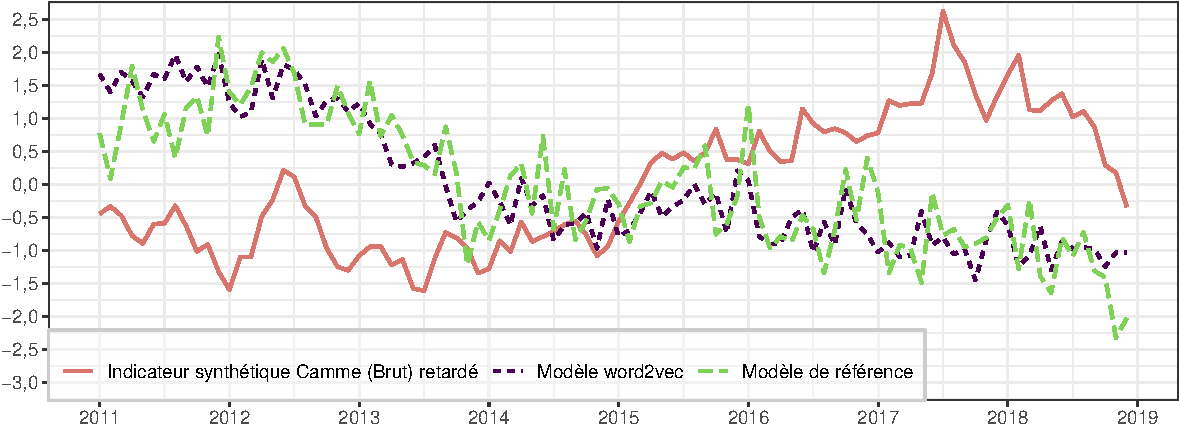
\includegraphics[width =0.7\textwidth]{img/rmd-graphSentiments-1}
\captionsetup{margin=0cm,format=hang,justification=justified}
\caption{Les trois indicateurs (centrés-réduits sur la période).}\label{fig:bslogcam}
\end{center}
\end{figure}

\begin{textblock*}{\textwidth}(5.5cm,-0.5cm)
\begin{center}
\begin{minipage}{0.7\textwidth}

\begin{wrapfigure}{L}{0cm}

\includegraphics[height=0.8cm]{img/avatars.png}
\end{wrapfigure}

$\phantom{saut}$

\emph{Retrouvez l'ensemble du projet et son code sur}

https://github.com/ARKEnsae/TweetEmbedding

\end{minipage}
\end{center}

\end{textblock*}

\end{document}
